\documentclass{beamer}

\title{Sommerfeld enhancement of dark matter signals at telescopes}
\author{Supervisor: Dr. Filippo Sala, Submitted by: Luca Zoppetti}
\institute{Alma Mater Studiorum - University of Bologna}
\date{22/07/2025}

\beamerdefaultoverlayspecification{<+->}

\graphicspath{ {../tex/images} }

\begin{document}

\frame{\titlepage}

\begin{frame}
\frametitle{Structure of the talk}
\begin{itemize}
	\item Dark matter evidence
	\item Indirect detection and Sommerfeld enhancement
	\item Quick mathematical review
	\item Results and conclusions
\end{itemize}
\end{frame}

\begin{frame}
\frametitle{Dark matter evidence (1): galaxy clusters}
In 1933, Fritz Zwicky estimated the velocity dispersion in the Coma cluster:
\[
	\sqrt{\langle v^2 \rangle } \simeq 80 \mathrm{km / s}
\]
\pause
The measured velocity dispersion along the line of sight is
\[
	v_{los} \sim 10^3 \mathrm{km / s} 
\]
\pause
Something doesn't add up!
\end{frame}

\begin{frame}
\frametitle{Dark matter evidence (1): galaxy clusters}
Use the virial theorem to estimate the mass in the cluster from known observational data:
\[
	\langle T \rangle = - \frac{1}{2} \langle U \rangle 
\]
\pause
% Known observational data:
% \begin{itemize}[<*>]
% 	\item \(v_{los} \sim 10^3 \mathrm{km / s} \)
% 	\item Distance is \(d \sim 100 \mathrm{Mpc} \)
% 	\item Angular radius is \(\theta \sim 1^{\circ } \)
% 	\item It is approximately spherically symmetric
% \end{itemize}
% \pause
We get
\[
	M \simeq 2 \times 10^{15} M_\odot
\]
\pause
It's off by one order of magnitude compared to the visible mass of \(10^{14} M_\odot\)!
\end{frame}

\begin{frame}
\frametitle{Dark matter evidence (2): galactic rotation curves}
From Newtonian mechanics, we expect
\[
	v(r) = \sqrt{\frac{GM(r)}{r}} 
\]
\pause
Observations by Rubin and Ford (1970), Roberts and Whitehurst (1975), and Carignan et al. (2006) show that velocity curves flatten at large radii.
\end{frame}

\begin{frame}
\frametitle{Dark matter evidence (2): galactic rotation curves}
\begin{figure}[htbp]
	\centering
	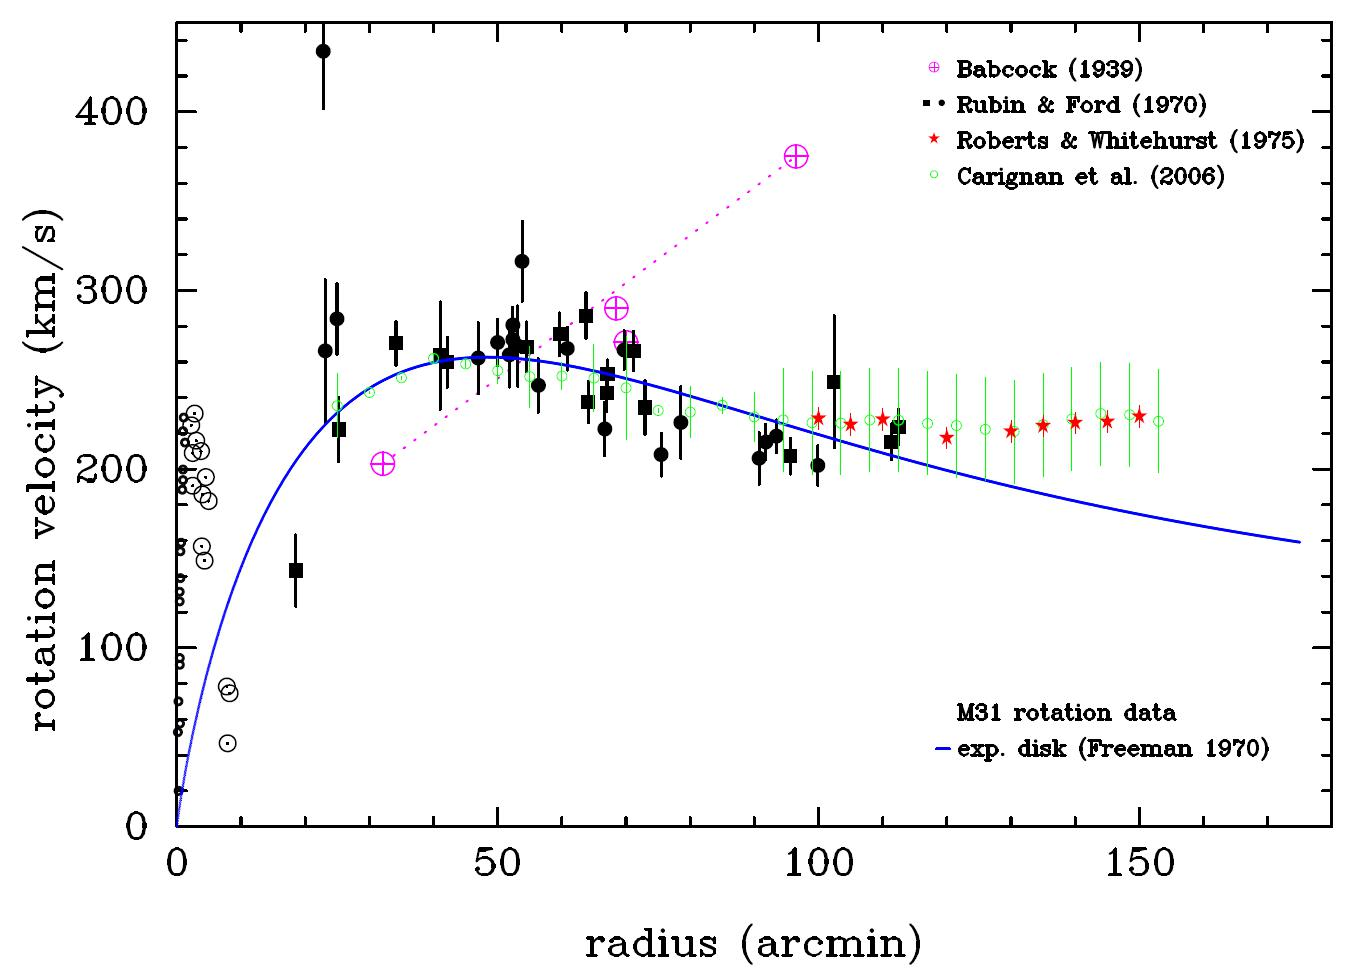
\includegraphics[width=0.8\textwidth]{rotation_curves.jpg}
	\caption{Rotational velocity data points for the M31 galaxy. In solid blue: theoretical prediction. Credits for the figure: Albert Bosma.}
	\label{fig:rotation_curves}
\end{figure}
\end{frame}

\begin{frame}
\frametitle{Dark matter evidence (2): galactic rotation curves}
The curve would flatten in the case of \(M \propto r\) at large radii. Several possible profiles exist (from simulations), NFW used in reference paper:
\[
	\rho_{\mathrm{NFW} } (r) = \frac{\rho _s}{\frac{r}{r_s} \left( 1+ \frac{r}{r_s} \right) ^2}
\]
\end{frame}

\begin{frame}
\frametitle{Dark matter evidence (3): the Bullet cluster}
\begin{figure}[htbp]
	\centering
	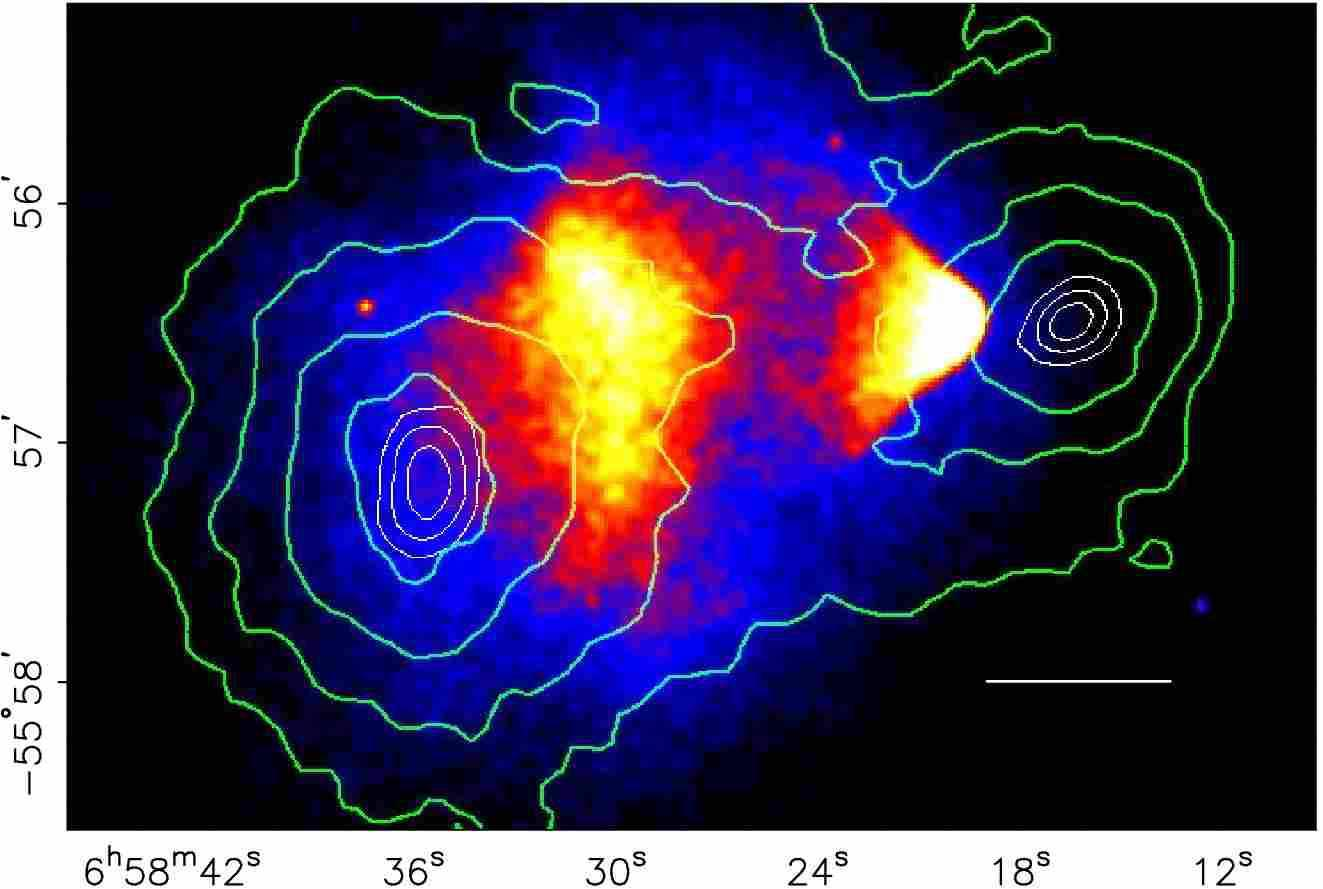
\includegraphics[width=0.8\textwidth]{bullet.jpg}
	\caption{The colormap shows X-ray-emitting matter. The green contours show the gravitational lensing signal. The two centres of mass are clearly displaced. Credits: Clowe et al. (2006).}
	\label{fig:bullet}
\end{figure}
\end{frame}

\begin{frame}
\frametitle{Dark matter evidence (4): CMB and large-scale structures}
The universe wouldn't look the way it does without dark matter:
\begin{itemize}
	\item It shaped the CMB acoustic peaks
	\item It acted as a catalyzer for large-scale structure formation (galaxies, clusters)
\end{itemize}
\pause
All of this evidence is independent and is explained at once by the hypothesis of dark matter!
\end{frame}

\end{document}